% !TeX spellcheck = de_DE
\section{Evaluation}
Nachdem die Parallelisierung der Evaluationsphase durchgeführt und die Testumgebung spezifiziert ist, wird in diesem Kapitel die Performance des Verfahrens gemessen. Die hierbei erhaltenen Ergebnisse werden mit denen der sequenziellen Implementierung verglichen. Im letzten Schritt wird eine Bewertung bezüglich der Effizient und des \emph{SpeedUps} abgegeben.

\subsection{Mountain Car}
Das parallelisierte Verfahren wird zuerst in der \emph{Mountain Car} Umgebung getestet, die aus Kapitel \ref{subsec:analysis_mountain_car} bekannt ist. Mit dem Ziel, einen einfachen Vergleich zwischen der sequenziellen und parallelisierten Implementierung zu ermöglichen, wird die zuvor verwendete Konfiguration des Verfahrens vollständig übernommen. Ebenfalls wird bei der Ausführung derselbe \emph{Seed} angegeben. Bei korrekter Implementierung des parallelisierten Verfahren werden dieselben Zwischenergebnisse nach jeder Generation generiert und auch das finale Ergebnis wird mit dem des sequenziellen Verfahren übereinstimmen. Somit kann keine Implementierung einen zeitlichen Vorteil erlagen, der durch bessere Agenten oder kürzere Evaluationszeiten entsteht. Beide Implementierungen werden dieselben Berechnungen und Evaluationen durchführen.
\begin{figure}[!h]
	\centering
	\begin{minipage}[]{0.49\textwidth}
		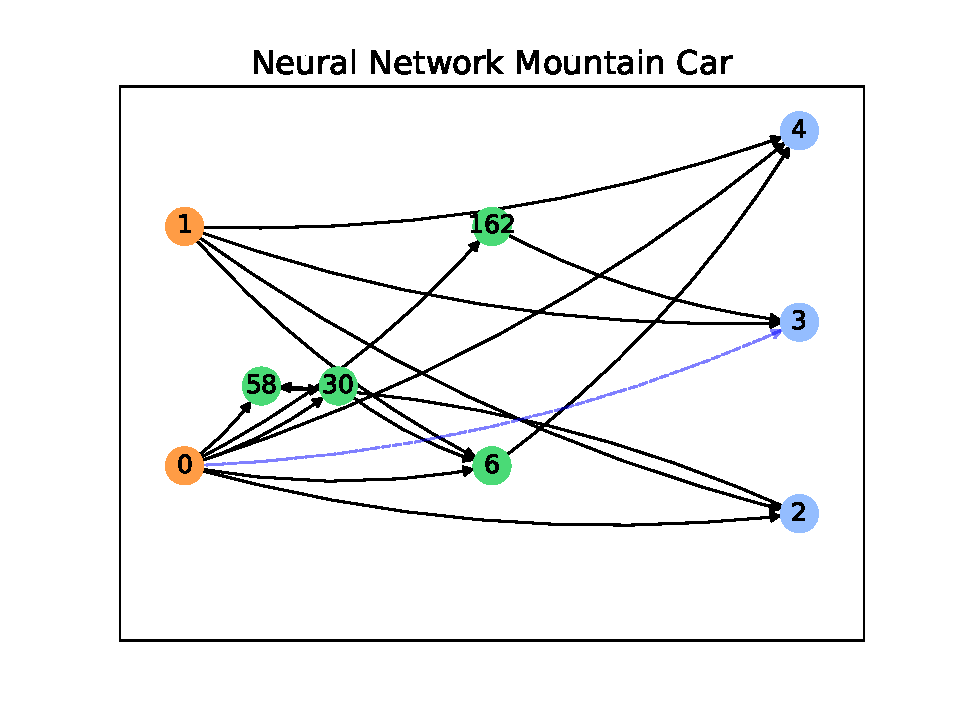
\includegraphics[width=1.0\textwidth]{./img/mountain_car_single/mountain_car_neural_network.pdf} 
	\end{minipage}
	\hfill
	\begin{minipage}[]{0.49\textwidth}
		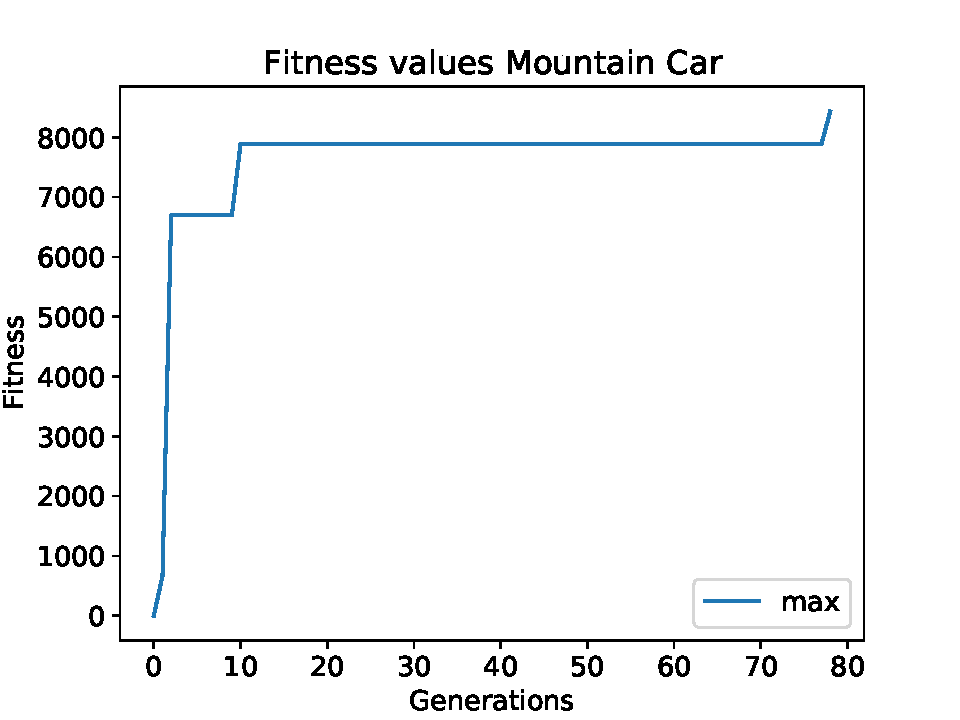
\includegraphics[width=1.0\textwidth]{./img/mountain_car_single/1413_fitness_1core_1pi.pdf} 
	\end{minipage}
	\caption{Links die Lösung für das Mountain Car Problem, rechts die dazugehörigen Fitnesswerte pro Generation mit 10 Prozessen}
	\label{fig:mountain_car_10core_neural_network_and_fitness}
\end{figure}
\\\\

\begin{figure}[!h]
	\centering
	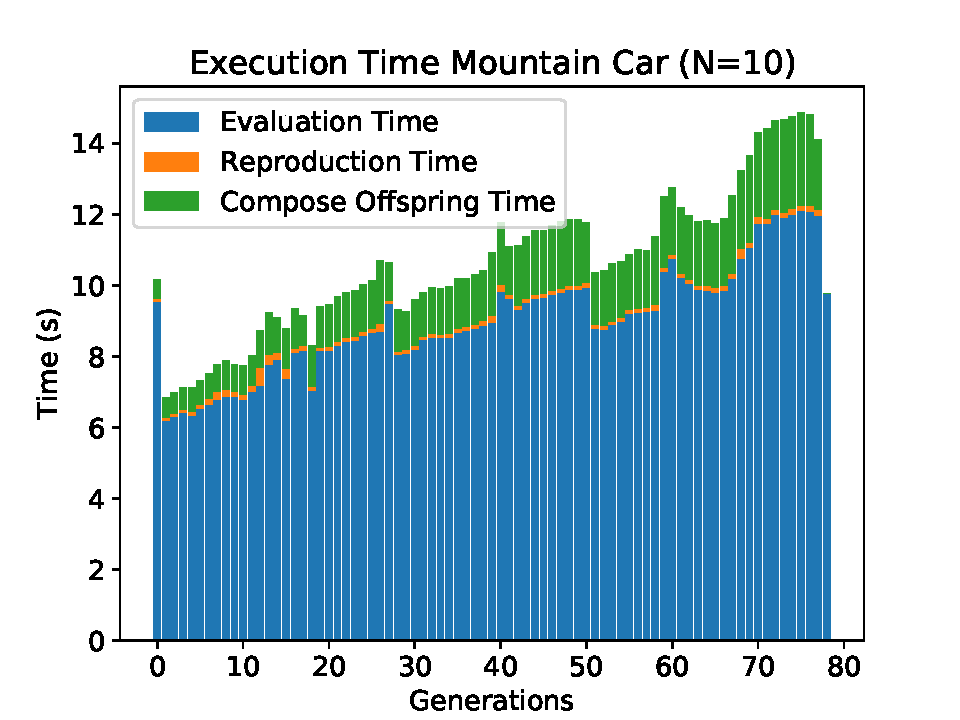
\includegraphics[width=0.7\textwidth]{./img/mountain_car_analysis/1413_time_10cores_10pis.pdf} 
	\caption{Ausführungszeit des \emph{Mountain Car} Problems auf 10 \emph{Raspberry Pis} mit 10 Prozessen}
	\label{fig:mountain_car_time_10cores_10pi}
\end{figure}

%\begin{figure}[!h]
%	\centering
%	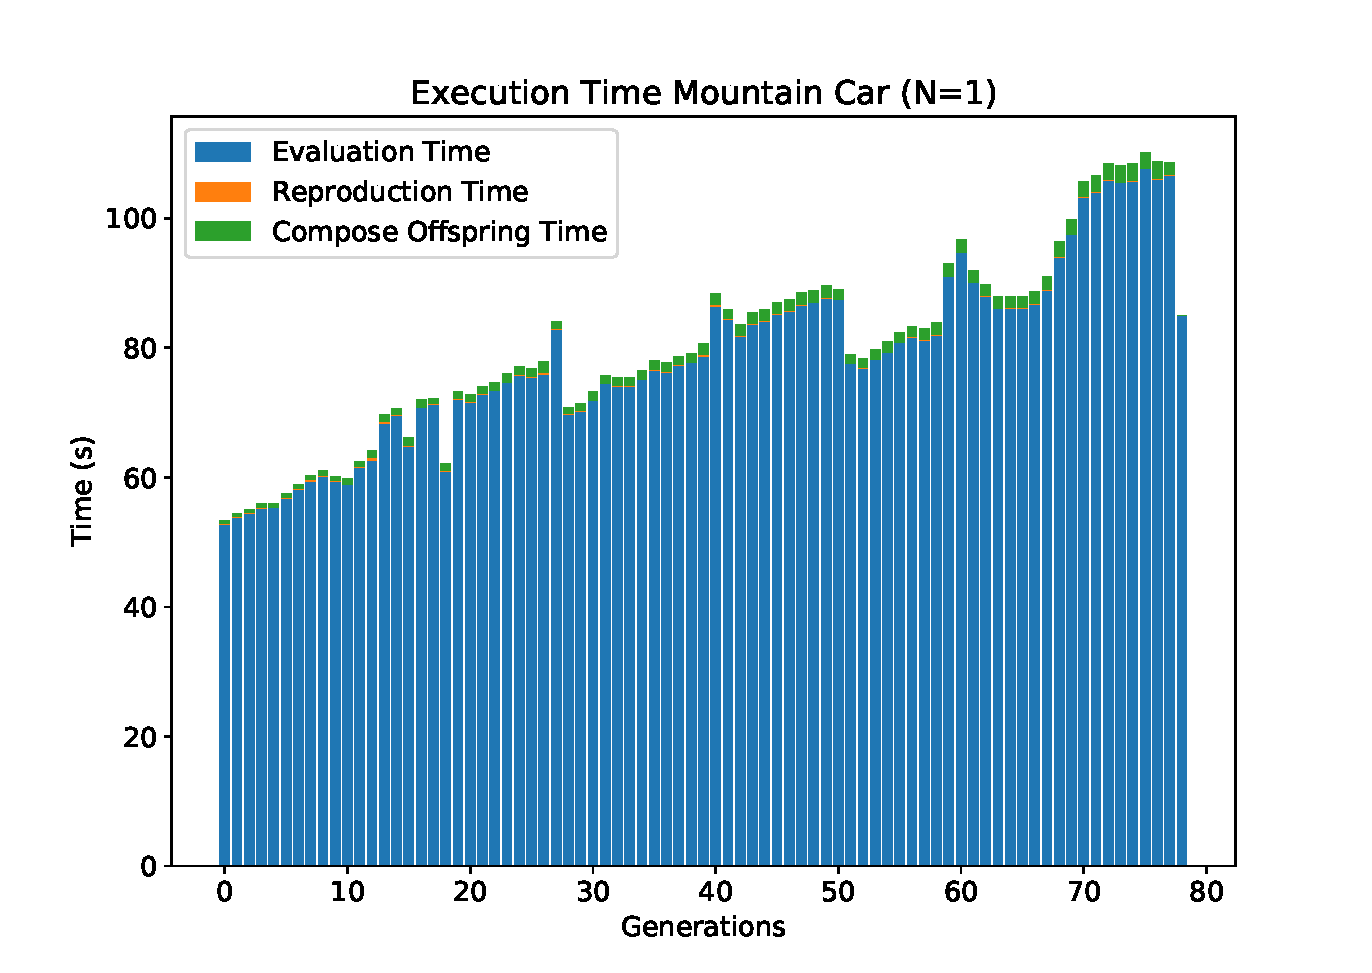
\includegraphics[width=0.7\textwidth]{./img/mountain_car_single/1413_time_1core_1pi.pdf} 
%	\caption{Ausführungszeiten des Mountain Car Problems auf einem Raspberry Pi 4 mit einem Prozess}
%	\label{fig:mountain_car_time_single_core}
%\end{figure}

% Compared to first: Total TIme: 840 sec (14min), EvaluationTIme : 712sec (11.8 min), Compose OffSpring 116.9, Reproduciton Time 10.7 Sekunden
% Total SpeedUp Compared to First  6341.262775421143 / 840 = Insgesamt 7.5, Evaluation, 7.5/10 = 75%   Time Faktor = 6218.207088708878 / 712 = 8.8 = 88%, mit 9 Cores 97% Effizienz

Im ersten Durchlauf wird der parallelisierte Algorithmus mit zehn Prozessen auf zehn Raspberry Pis ausgeführt. Das Verfahren ist so konfiguriert, dass auf jedem Raspberry Pi ein Prozess gestartet wird. Abbildung \ref{fig:mountain_car_10core_neural_network_and_fitness} zeigt das hierbei entstandene \ac{KNN} und den maximal erreichten Fitnesswert. Beide Darstellungen sind identisch zu denen des sequenziellen Verfahrens. Da auch die restlichen Zwischenergebnisse stimmen über ein, wie beispielsweise die Anzahl an verschiedenen Spezies pro Generation, ist die Anforderung bezüglich des \emph{Seeds} erfüllt. Sowohl die parallelisierte als auch die sequenzielle Implementierung führen dieselben Rechenschritte durch, womit ein direkter Vergleich der Laufzeiten möglich ist. Die Ausführungszeit für die vorgestellte Konfiguration ist in Abbildung  \ref{fig:mountain_car_time_10cores_10pi} dargestellt. Wie bei dem sequenziellen Verfahren wird die diese in die Phasen \emph{Evaluation Time}, \emph{Reproduction Time} und \emph{Compose Offspring Time} unterteilt. Grundsätzlich ist festzustellen, dass die insgesamt benötigte Laufzeit stark verringert ist. Mit zehn Prozessen in der vorgestellten Konfiguration sinkt die durchschnittliche Rechenzeit auf ungefähr $10.5$ Sekunden pro Generation. Die sequenzielle Implementierung hat im Vergleich dazu etwa $80$ Sekunden pro Generation benötigt. Für die gesamten Ausführungszeit des Verfahrens bedeutet dies, dass das parallelisierte Verfahren bereits nach $14$ Minuten beendet wird. Im Vergleich zur Laufzeit der sequenziellen Implementierung mit $105$ Minuten ist das parallelisierte Verfahren somit $91$ Minuten schneller.
\\\\
Eine Besonderheit des Graphen zeigt sich in der ersten Generation. In dieser ist die Ausführungszeit der \emph{Evaluation Time} vergleichsweise hoch. Der Grund hierfür ist, dass das Starten und Initialisieren der beteiligten Prozesse Zeit benötigt, welche die Evaluation der Agenten verzögert. Da dies im Rahmen der \emph{Evaluation Time} erfasst wird, erhöht sich die gemessene Ausführungszeit in der ersten Generation. Für die nachfolgenden Generationen trifft dies nicht mehr zu, da die Initialisierung nur einmalig zu Beginn erfolgt. Eine weitere Besonderheit betrifft die Form des Graphen. Wie bei der sequenziellen Implementierung gibt es auch in der parallelisierten Implementierung Generationen, in der die Ausführungszeit stark sinkt oder ansteigt. Mögliche Gründe hierfür sind im Kapitel \ref{subsec:analysis_mountain_car} erörtert. Bei einem direkten Vergleich der Ausführungszeiten ist festzustellen, dass diese Änderungen meistens in denselben Generationen auftreten. Diese Eigenschaft ist wichtig, da ein Vergleich der Laufzeiten nur möglich ist, wenn die Messergebnisse, abgesehen von kleinen Abweichungen, konsistent sind. Dies Eigenschaft kann zusätzlich mit der \emph{Reproduction Time} und \emph{Compose Offspring Time} verifiziert werden. Diese Phasen sind nicht parallelisiert und daher sollte die Ausführungszeit identisch sein. Insgesamt sind die gemessenen Laufzeiten dieser Phasen etwas höher als bei der sequenziellen Implementierung. Über die $78$ Generationen entsteht eine Differenz von ungefähr $5$ Sekunden beziehungsweise $4\%$. Diese Unterschiede können beispielsweise durch Hintergrundprozesse im Betriebssystem entstehen, auf welche kein Einfluss genommen werden kann. Da die Abweichungen insgesamt gering sind, kann trotzdem ein Vergleich der Laufzeiten durchgeführt werden. Der letzte zu nennende Eigenschaft bezüglich der Abbildung \ref{fig:mountain_car_time_10cores_10pi} ist der prozentuale Anteil der \emph{Reproduction Time} und \emph{Compose Offspring Time}. Bei der sequenziellen Implementierung haben diese beiden Phasen nur etwa $2\%$ der Ausführungszeit ausgemacht. Dadurch dass der Anteil \emph{Evaluation Time} durch die Parallelisierung gesunken ist, steigt der Anteil auf ungefähr $15$ an. \emph{Amdahl's Law} entsprechend wird dieser Anteil mit weiteren Prozessen zunehmen.
\begin{figure}[!h]
	\centering
	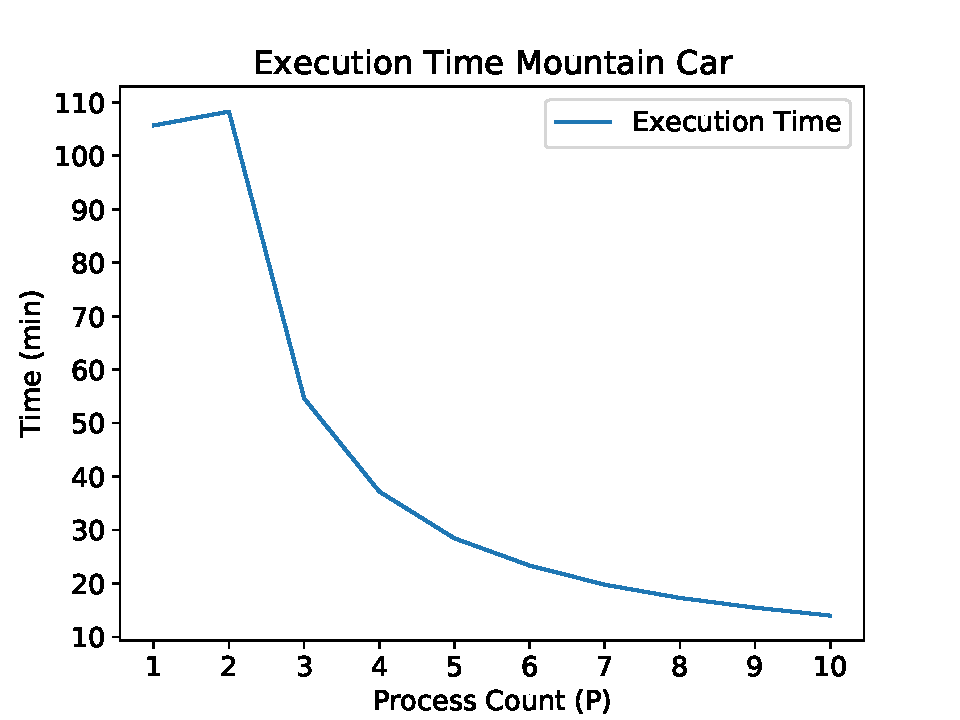
\includegraphics[width=0.7\textwidth]{./img/mountain_car_analysis/time_mountain_car_1_10.pdf} 
	\caption{Ausführungszeit des parallelisierten Verfahrens in der \emph{Mountain Car} Umgebung in Abhängigkeit der Prozessanzahl}
	\label{fig:execution_time_mountain_car_1_10}
\end{figure}
\\\\
Für eine vollständige Bewertung des parallelisierten Verfahrens werden die in Kapitel \ref{subsec:basics_performance} vorgestellten Metriken \emph{SpeedUp} und Effizienz benötigt. Für eine bessere Einordnung der Ergebnisse, werden diese nicht nur für die oben vorgestellte Konfiguration mit zehn, sondern auch für Testdurchläufe mit zwei bis neun Prozessen berechnet. Diese werden im Folgenden mit derselben Konfiguration durchgeführt. Die hierbei entstehenden \ac{KNN} und Fitnesswerte sind identisch zu den Vorherigen und daher nicht abgebildet. Die benötigte Ausführungszeit für das gesamte Verfahren in Abhängigkeit der Anzahl an Prozessen ist in Abbildung \ref{fig:execution_time_mountain_car_1_10} dargestellt. Eine Besonderheit hierbei ist, dass die Ausführungszeit mit zwei Prozessen länger benötigt als mit einem Prozess. Der Grund hierfür liegt in der gewählten \emph{Master-Slave} Architektur des parallelisierten Verfahrens. Mit einem Prozess wird das sequenzielle und andernfalls das parallelisierte Verfahren ausgeführt. Werden genau zwei Prozesse verwendet, gibt es einen \emph{Master} und einen \emph{Slave}. In diesem Fall ist die Ausführung langsamer als das sequenzielle Verfahren, da der \emph{Master} im Rahmen der Parallelisierung nur die Kommunikation koordiniert und selbst keine Aufgabenpakete abarbeitet. Der \emph{Slave} muss alleine die Evaluationen der Agenten durchführen. Dafür benötigt er dieselbe Zeit wie das sequenzielle Verfahren. Hinzu kommt der benötigte Kommunikationsaufwand, der für das Verteilen von Agenten und Sammeln von Fitnesswerten benötigt wird. Die hierfür benötigte Zeit macht das parallelisierte Verfahren mit zwei Prozessen langsamer als das sequenzielle Verfahren. Mit drei oder mehr beteiligten Prozessen sinkt die Ausführungszeit kontinuierlich. 
\\\\
Anhand der Ausführungszeiten kann der \emph{SpeedUp} und die Effizienz des parallelisierten Verfahrens gemessen werden. Mit diesen letztendlich eine Bewertung der Implementierung möglich. Abbildung (TODO ABBILDUZNG) zeigt links den erreichten \emph{SpeedUp} und rechts die dazugehörigen Effizienzwerte in Abhängigkeit der Anzahl an verwendeten Prozessen.  

\begin{figure}[!h]
	\centering
	\begin{minipage}[]{0.49\textwidth}
		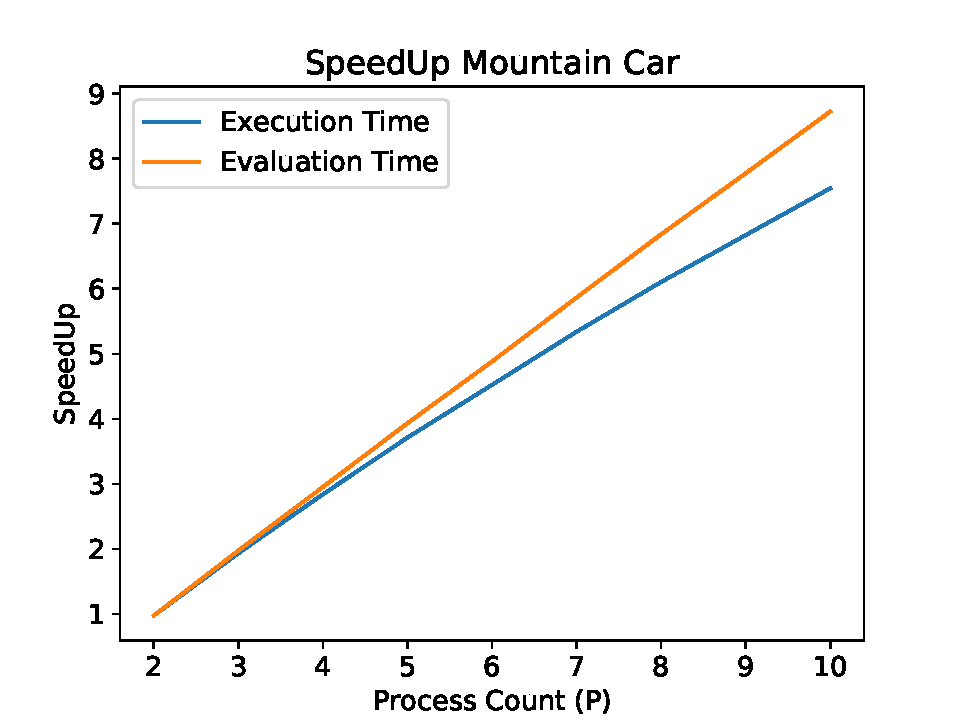
\includegraphics[width=1.0\textwidth]{./img/mountain_car_analysis/mountain_car_speedup_2_10.pdf} 
	\end{minipage}
	\hfill
	\begin{minipage}[]{0.49\textwidth}
		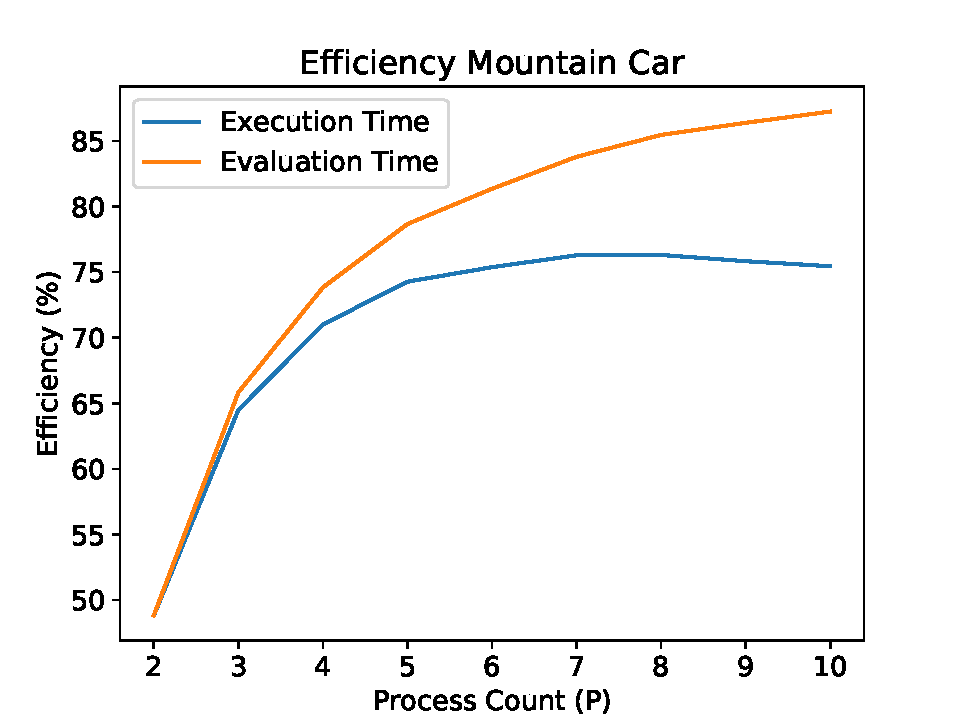
\includegraphics[width=1.0\textwidth]{./img/mountain_car_analysis/efficecny mountain_car_2_10.pdf} 
	\end{minipage}
	\caption{Links die Lösung für das Mountain Car Problem, rechts die dazugehörigen Fitnesswerte pro Generation mit 10 Prozessen}
	\label{fig:mountain_car_2_10_efficiency_speedup}
\end{figure}

%\begin{figure}[!h]
%	\centering
%	\includegraphics[width=0.7\textwidth]{./img/mountain_car_analysis/mountain_car_speedup_1_10.pdf} 
%	\caption{\emph{SpeedUp} des parallelisierten Verfahrens}
%	\label{fig:speedup_mountain_car_1_10}
%\end{figure}

% Prozentsatz an Abweidung nicht parllelisierter Verfahren, 
% Zuerst Ergebnisse 10 Pis, mit Verifizierung Funktionalität und allgemeines Ergebnis
% Eingehen dass Master Pi keine Abarbeitugn übernimmt sondern nur Koordination
% Zeiten von anderen Phasen weichen ab, daher kann es zu varianzen kommen
% Allgemeine Laufzeit des Verfahrens und Laufzeit des evaluierten Verfahren anzeigen
% Vergleich mit Amdahls Law? +++++ 
